\documentclass[
	a4paper,
    headings=small,  % kleinere Überschriften
    oneside,        % einseitig, nur rechte seiten
    listof=totoc,   % listen in inhaltsverzeichnis aufnehmen
    bibliography=totoc,  % literaturverzeichnis in inhltsvz. aufnehmen
    headsepline     % trennlinie unter kopfzeile
    ]{scrbook}
    
\usepackage[utf8]{inputenc}

%Verwende deutsche, bzw. amerikanische Silbentrennung
\usepackage[ngerman]{babel} 

\usepackage{subfig} %für mehrteilige Grafiken
\usepackage{epsfig}    %damit funktioniert das einbinden von grafiken über epsfig.
\usepackage{graphicx}     % zum einbinden von grafiken
\usepackage{svg}
\graphicspath{{grafiken}{../}{kapitel}} %da sind mögliche bilder fuer den includegraphics-Befehl zu finden (man muss dann nicht den ganzen Pfad bei includegraphics angeben.
\usepackage{color} % um Farben benutzen zu können
\usepackage{breakcites} %damit Literaturangabe (cite-Befehl) im Text umgebrochen wird
\usepackage{multirow}     %fuer kompliziertere Tabellen
\usepackage{framed}
\usepackage{url}
\usepackage{tikz}
\usetikzlibrary{decorations.pathreplacing,angles,quotes}
\usepackage{scrlayer-scrpage}     % paket für kopf- und fu{\ss}zeilen
\pagestyle{scrheadings}   % kopzeilenseitenstil
\usepackage{natbib}       % Literaturverzeichnis
\usepackage{amsmath,amsfonts,amssymb}

\setlength{\parindent}{0pt}
\setlength{\parskip}\medskipamount % besser als explizite Angabe in pt

% kapitelüberschriften in schriftart mit serifen
\setkomafont{sectioning}{\normalfont\normalcolor\bfseries}

% gestaltung der kopfzeilen
\ohead{\pagemark}
\cfoot{}
\cohead{}
\ihead{\headmark}
\setkomafont{pageheadfoot}{\normalfont \bfseries}
\setkomafont{pagenumber}{\normalfont \bfseries}
\automark{section}

\begin{document}
\selectlanguage{ngerman} %deutsche Silbentrennung
\frontmatter      % vorspann, kapitel römisch nummeriert
% Die Titelseite der Arbeit

\begin{titlepage}

\begin{center} % zentrieren

  % Logo der Universität Mainz
  \begin{figure}[ht]
    \centering
    
\includegraphics{grafiken/jogu_logo.eps}
  \end{figure}

  % Vertikaler Zwischenraum
  \bigskip
  \vfill
  \begin{framed}
  % Titel der Arbeit und Typ der Arbeit, umrandet
    \begin{center}
      \textsc{{\Large Klassifikation elektrischer Muskelaktivität durch Tiefe Neuronale Netze\\}}
                                % Letztes \\ ist wichtig, beginnt eine neue Zeile f{\"u}r die Art der Arbeit

      \bigskip

                                % Art der Arbeit, ggf. auszutauschen gegen Seminar- oder Doktorarbeit
      \textbf{Bachelorarbeit}
    \end{center}
    \end{framed}
    \vfill
    \vfill

  % Daten des Erstellers, Einreichungsdatum
  % in einer Tabelle ausgerichtet
  \begin{tabular*}{0.62\textwidth}{r@{\extracolsep{\fill}}l}
    eingereicht im: & August 2020\\\\
    von: & Alexander Seidmann\\
    & geboren am 22. Januar 1998\\
    & in Frankfurt am Main\\
    \\
    Matrikelnummer: & 2740392\\
    \\
    Betreuer: & Dr. Paul Kaufmann
  \end{tabular*}
  \vfill
  \vfill

  % Unten: Kontaktdaten des Lehrstuhls f�r Wirtschaftsinformatik und BWL

  \rule{\textwidth}{.4pt}\\ % vertikale Linie
  Johannes Gutenberg-Universität Mainz\\
  Fachbereich Rechts- und Wirtschaftswissenschaften\\
  Lehrstuhl für Wirtschaftsinformatik und BWL\\
  Telefon: +49 6131 39-22734, Fax +49 6131 39-22185\\
  Internet: \url{http:///wi.bwl.uni-mainz.de}
\end{center}

\end{titlepage} % Ende des Titelblatts

     % titelseite einbinden
\tableofcontents            % inhaltsverzeichnis
\listoffigures              % abbildungsverzeichnis
\listoftables               % tabellenverzeichnis
%-------------------------------------
%
%    minimales abk�rzungsverzeichnis
%
%-------------------------------------

\addchap{Abk\"{u}rzungsverzeichnis} % beachte addchap
\begin{labeling}{1234567890}
        \item[BP] Backpropagation 
        \item[BTT] Backpropagation Through Time
        \item[BZ] Batch Size
        \item[CS] Cell State
        \item[DNN] Tiefe Neuronale Netze
        \item[DT] Entscheidungsbäume
        \item[EG] Exploding Gradient
        \item[EG] Exploding Gradient        
        \item[EMG] Oberflächenmyographie 
        \item[ES] Eingebettete Systeme
        \item[FD] Frequenzbereich 
        \item[FGL] Forget Gate Layer
        \item[GC] Gradient Clipping
        \item[GD] Gradientenabstieg
        \item[GRU] Gated Recurrent Unit
        \item[HL] Hidden Layer
        \item[HS] Hidden State 
        \item[IGL] Input Gate Layer
        \item[LN] Leaf Nodes
        \item[LR] Lernrate
        \item[LSTM] Long Short Term Memory
        \item[MAV] Mean Absolute Value
        \item[MLP] Multi Layer Perceptron
        \item[OGL] Output Gate Layer
        \item[RG] Reset Gate
        \item[RG] Reset Gate  
        \item[RNN] Rekurrente Neurale Netze
        \item[ReLU] Rectified Linear Unit
        \item[SGL] State Gate Layer
        \item[SM] Soft Margin                              
        \item[SSC] Slope Sign Changes
        \item[SVM] Support Vector Machines
        \item[SV] Support Vectors
        \item[TD] Zeitbereich
        \item[UG] Update Gate
        \item[UG] Update Gate
        \item[VG] Vanishing Gradient
        \item[VG] Vanishing Gradient
        \item[WL] Waveform Length
        \item[ZC] Zero Crossing
        \item[kNN] k Nearest Neighbors
        \item[kNN] k nächste Nachbarn 
        \item[sEMG] Oberflächen-Elektromyografie
\end{labeling}   % beispiel eines handerstellten
                                %verzeichnisses
\mainmatter       % hauptteil, kapitel lateinisch nummeriert
\chapter{Einleitung}
\label{chap:einleitung}

Seit einigen Jahren sind Tiefe Neuronale Netze (DNN) bereits ein etablierter Teilbereich der
Forschung an künstlicher Intelligenz. So spielen DNN in einer Vielzahl von
Anwendungsbereichen eine stetig wachsende Rolle.
Durch die Weiterentwicklung der den DNN zugrunde liegenden Algorithmen und der für die
Implementierung verwendeten Hardware verzeichnen diese Technologien jüngstens auch in
Bereichen wie der Klassifikation von elektrischer Muskelaktivität erhebliche Fortschritte (\cite{Allard2019}). Hierfür ist
eine gängige Methode die Verwendung von Oberflächen-Elektromyografie (sEMG), bei der
äußerlich an der Haut angebrachte Elektroden die elektrischen Impulse der darunter befindlichen
Muskulatur messen und aus diesen Merkmale für die Klassifikation extrahieren. Durch die Klassifikation der Merkmale kann somit dem Impuls eine korrespondierende Bewegung zugeordnet werden. Diese Möglichkeit der Informationsextraktion und Umwandlung ist besonders im Bereich der Prothesik interessant, da so Menschen mit fehlenden Gliedmaßen eine Prothese mithilfe ihrer natürlichen Muskelkontraktionen steuern können. Die Verwendung solcher Klassifikatoren mit hohen rechnerischen Anforderungen, war zuvor laut \cite{Allard2019} in den aufgrund ihres Anwendungsbereichs leistungsschwachen eingebetteten Systemen (ES) nahezu unmöglich (\cite{Allard2019}).
Da bei der Klassifizierung von zwischen einzelnen Aufnahmen stark variierenden
elektrischen Daten Anpassbarkeit eine wichtige Kerneigenschaft ist (\cite{Kaufmann2013}), öffnet die
Verwendung von durch Daten stetig lernenden DNN eine ideale Grundlage für die
Weiterentwicklung solcher Technologien.

\section{Ziel der Arbeit}

Ein Forschungsschwerpunkt der vorigen Jahre waren im Bereich der Klassifikation elektrischer Muskelaktivität die Rekurrenten Neuralen Netze (RNN) (\cite{simao2019emg}, \cite{tsuji2000pattern}). Solche Netze sind vor allem für die Klassifikation und Regression von Daten mit einer zeitlichen Dimension effektiv, da sie anders als andere gängige Neurale Netze anstatt von Momentaufnahmen sequentielle Daten analysieren und klassifizieren können. Solche Architekturen zeigten sich bereits in vorherigen Untersuchungen in der Klassifikation von EMG-Signalen gute Ergebnisse (\cite{simao2019emg}).

Ziel dieser Arbeit ist der Vergleich von RNN mit anderen gängigen Klassifikatoren im Bereich der EMG-Signale durch die Untersuchung auf einem sEMG-Datensatz. RNN unterliegen in ihrer einfachsten Form häufig dem vanishing Gradient Problem, wodurch anfängliche Daten das Ergebnis einer einzelnen Klassifikation immer weniger beeinflussen, je weiter das Netzwerk in der Klassifikation der Sequenz fortschreitet (\cite{pascanu2013difficulty}). Auf Grund dieser Problematik werden für den Vergleich zwei Weiterentwicklungen des normalen RNN, die Architekturen \textit{long short term memory} (LSTM) und \textit{gated recurrent unit} (GRU), zusätzlich herangezogen, um unter der Verwendung von state-of-the-art Architekturen sowohl präzisere als auch repräsentativere Ergebnisse zu erzielen. Die Netzwerkarchitekturen werden mit gängigen Algorithmen verglichen, die in der Vergangenheit bereits gute Ergebnisse in der Klassifikation vom EMG-Signalen erzielt haben. (\cite{Kaufmann2013}) Herangezogen werden \textit{k nearest neighbors} (kNN), \textit{support vector machines} (SVM), \textit{decision trees} (DT) sowie ein \textit{multi layer perceptron} (MLP), also eine einfache Form eines Neuralen Netzwerks.
Die Architekturen und Algorithmen werden stets mit dem durch \cite{Kaufmann2013Data} erhobenen Datensatz "Forearm EMG 121" trainiert und getestet. Hier handelt es sich um die Aufnahmen von elf Handbewegungen über einen Zeitraum von 21 Tagen. Die Aufnahme erfolgte dabei durch ein am Unterarm platziertes Armband über vier Aufnahmepunkte, aus deren Zeitbereich die Merkmale für den Datensatz extrahiert wurden. Alle untersuchten Architekturen und Algorithmen werden mit demselben Datensatz trainiert und getestet, wobei der Datensatz aufgrund der sequentiellen Natur von RNN für diese in Sequenzen unterteilt wird.

Diese Arbeit soll die Grundlage für weitere Forschung in diesem Bereich der Klassifikation von EMG-Signalen bilden, indem Referenzwerte erhoben und im Vergleich dargestellt werden.


\section{Aufbau der Arbeit}
\label{sec:aufbau-der-arbeit}

% EMG-Signale und Merkmalsextraktion
Zunächst erfolgt im zweiten Kapitel eine Einführung in die Messung von elektischer Muskelaktivität durch sEMG und die daraus abzuleitende Merkmalsextraktion.
% Der verwendete Datensatz
Weiterhin wird im folgenden Kapitel der fortlaufend verwendete Datensatz in Bezug auf die Anforderungen, Eigenschaften, Klassen und die extrahierten Merkmale präsentiert.
% Einführung Tiefe Neuronale Netze
Sobald der Grundstein für ein Verständnis der Daten gelegt ist, folgt ein kurzer
Einblick in die Funktionsweise von Neuralen und tiefen Neuralen Netzen im Allgemeinen, wobei ihr bisheriger Einsatz in der Klassifikation von EMG Signalen betrachtet wird.
% Experimentaler Aufbau
Im fünften Kapitel wird der Experimentelle Aufbau aufgezeigt und die Rahmenbedingungen beschrieben. 
% Recurrent Neural Networks
Daraufhin wird die
Funktionsweise von RNN erläutert, wobei hier zunächst die Besonderheiten der Architektur und die Problematik des vanishing und exploding Gradient eingegangen wird. Anschließend werden die angewandten Architekturen zur Lösung selbiger, LSTM und GRU, ebenfalls vorgestellt und beschrieben, wie diese die Nachteile gewöhnlicher RNN Strukturen umgehen.
% Andere Klassifikatoren
Das siebte
Kapitel beleuchtet die Architekturen und Algorithmen, die für den Vergleich mit den RNN verwendet werden. Somit wird auf MLP, kNN, SVM sowie DT eingegangen und deren Funktionsweise erläutert.
% Ergebnisse und Vergleich
Im vorletzten Kapitel werden die Ergebnisse der einzelnen Klassifikatoren vor- und ein Vergleich aufgestellt, bevor im finalen Kapitel ein Fazit und
Ausblick die Arbeit konkludieren.

% EMG-Signale und Merkmalsextraktion ✅
% Der verwendete Datensatz ✅
    % Anforderungen ✅
    % Eigenschaften, Klassen und Merkmale ✅
% Einführung Tiefe Neurale Netze
% Recurrent Neural Networks
    % Einführung Recurrent Neural Networks
    % Einführung Long Short Term Memory
    % Einführung GRU
% Andere Klassifikatoren
    % Multi Layer Perceptron
    % k nearest Neighbors
    % Support Vecor Machines
    % Decision Trees
% Ergebnisse und Vergleich
% Zusammenfassung und Ausblick

\chapter{EMG-Signale und Merkmalsextraktion}
\label{chap:emg}

% Elektromyographie ist ein Verfahren zur Messung elektrischer Muskelaktivität ✅
% Impuls wird vom Hirn bis zur motorischen Endplatte weitergeleitet, auf der unterschiedliche Ionen ausgeschüttet werden ✅
% Es entstehen kleine messbare Zuckungen im Muskel ✅
% Messung entweder intramuskulär (aufwändig, aber weniger Rauschen) oder von außen mit Trocken- oder Gelelektrode ✅
% In der Praxis vor allem äußere Messung mit Trockenelektroden relevant ✅

Nach \cite{bischoff2015emg} wird elektrische Muskelaktivität wird durch kleine Zuckungen im Muskel ausgelöst, sobald ein Signal vom Gehirn aus die Anweisung für eine Bewegung sendet. Die Messung dieser Signale bezeichnet man als Elektromyographie. Hierbei ist die Art der Messung essenziell für eine qualitativ hochwertige Auswertung der Signale. So unterscheidet man beispielsweise zwischen intramuskulärer Messung und der Messung über extern an der Haut angebrachte Elektroden. Während die Messung von EMG-Signalen über intramuskuläre Elektroden genauer ist als eine duch die Anbringung der Elektroden auf der Haut, da externe Störfaktoren wie die Beschaffenheit der Haut ausgeschlossen werden können, sind diese alltagstauglicher und finden somit in der Praxis häufiger Anwendung (\cite{bischoff2015emg}). Hier kann man laut \cite{Allard2019} weiterhin zwischen Gel- und Trockenelektroden unterscheiden. Bei diesen verhält es sich ähnlich wie bei dem Vergleich der intramuskulären und äußeren Messung. Während Gelelektroden rauschfreiere Signale liefern, sind diese aufgrund der vorbereitenden Maßnahmen für eine alltägliche Nutzung in der Regel nicht geeignet (\cite{Allard2019}). Deshalb tendiert man häufig auch hier in der Anwendung zu den alltagstauglichen Trockenelektroden. Die Messung von Elektromyographischen Signalen über an der Haut angebrachte Elektroden bezeichnet man dabei als \textit{Oberflächen-Elektromyographie} (sEMG) (\cite{bischoff2015emg}).

Um nun mit Hilfe von Algorithmen oder Neuralen Netzen die sEMG-Signale zu klassifizieren, müssen Merkmale extrahiert werden. Der Zweck von Merkmalen ist es nach \cite{zecca2002control}, vergleichbare Eigenschaften der Signale zu erhalten und gleichzeitig für die Klassifikation überflüssige Daten herauszufiltern. Das ist relevant, da für eine erfolgreiche Klassifikation sowohl ausreichend aussagefähige Daten als auch eine hohe rechnerische Effizienz von Nöten sind.  Meistens muss diese Merkmalsextraktion vor dem Einspeisen der aufgezeichneten Daten ins Netz geschehen (\cite{zecca2002control}). Eine Ausnahme hiervon bilden die sogenannten Convolutional Neural Networks, die die Merkmalsextraktion innerhalb der Netzwerkarchitektur vornehmen (\cite{Allard2019}). Sämtliche in dieser Arbeit besprochenen Klassifikatoren benötigen bereits extrahierte Merkmale als Eingabewerte, weshalb im Folgenden auf die verschiedenen Bereiche und Unterschiede in der Merkmalsextraktion eingegangen wird.

So unterscheidet man bei der Merkmalsextraktion zwischen der Extraktion aus dem Zeit-, Frequenzbereich oder einer Mischung aus beiden (\cite{zecca2002control}).

Laut \cite{zecca2002control} finden die Merkmale aus dem Zeitbereich (TD) aufgrund ihrer hohen rechnerischen Effizient häufig Anwendung. Dieser stellt durch einen Graphen die Entwicklung von elektrischer Spannung in Abhängigkeit von Zeit dar. Die rechnerische Effizienz ist darauf zurückzuführen, dass es für die Merkmalsextraktion aus dem TD keiner Transformation bedarf (\cite{zecca2002control}). Für die Klassifikation von sEMG Signalen werden in dieser Arbeit die Merkmale des \textit{mean absolute value}, des \textit{zero crossings}, des \textit{slope sign changes} und der \textit{waveform length} entnommen, da diese in der Forschung bereits zu guten Ergebnissen führten (\cite{Engelhart2003}, \cite{Kaufmann2013}). Die extrahierten Merkmale werden im Detail im nächsten, den Datensatz thematisierenden, Kapitel beschrieben.

Der \textit{Frequenzbereich} (FD) betrachtet nach \cite{zecca2002control} anders als der TD die elektrische Spannung in Abhängigkeit der Frequenz. Um aus dem FD Merkmale zu extrahieren, müssen die Daten aus diesem zunächst transformiert werden. Das macht die Merkmalsextraktion rechnerisch intensiver als die Extraktion aus dem TD, weshalb diese Methode seltener für die Klassifikation von sEMG-Signalen in ES verwendet wird (\cite{zecca2002control}).

Eine weitere Möglichkeit der Merkmalsextraktion ist die Kombination von Zeit- und Frequenzbereich (\cite{zecca2002control}).
% Nochmal in den Quellen überprüfen
Hier wird die elektrische Spannung nicht nur in Abhängigkeit von Zeit, sondern auch in Abhängigkeit der Frequenz betrachtet. Daraus resultiert eine größere Vielfalt an Merkmalen, allerdings ist für die Extraktion trotzdem eine Transformation nötig, weshalb dieser Prozess rechnerisch ebenfalls intensiver ist als die direkte Extraktion aus dem Zeitbereich (\cite{zecca2002control}). 
% !TEX root = ../dnn_ba.tex
\chapter{Der verwendete Datensatz}
\label{chap:datensatz}

Dieses Kapitel beleuchtet den in der Forschungsarbeit verwendeten Datensatz. Hierfür wird zunächst erläutert, welche Eigenschaften der Datensatz erfüllen muss, damit die Ergebnisse der Arbeit auf die praktische Anwendung übertragbar sind. Im Zuge dessen werden die Anforderungen aufgelistet und es wird kurz erläutert, wie diese durch den vorliegenden Datensatz erfüllt werden.
Weiterhin wird auf die Aufzeichnung und Merkmalsextraktion des Datensatzes eingegangen, die darin enthaltenen Klassen vorgestellt und die aus dem Zeitbereich extrahierten Merkmale im Detail besprochen.

\section{Anforderungen an den Datensatz}

Der Prozess der Klassifikation und Zuordnung eines EMG-Signals zur dazugehörigen Bewegung kann in drei Schritte unterteilt werden:

\begin{itemize}
	\item die \textbf{\textit{Merkmalsextraktion}},
	\item die \textbf{\textit{Dimensionsreduktion}}
	\item und die \textbf{\textit{Musterklassifikation}}
\end{itemize}

Während man sich in der Praxis mit der Optimierung aller drei Phasen beschäftigen muss, liegt der Fokus dieser Arbeit auf der Musterklassifikation eines bereits durch \cite{Kaufmann2013Data} präparierten Datensatzes. Da daher die nachträgliche Manipulation der Merkmalsextraktion und Dimensionsreduktion ausgeschlossen ist, müssen im vorliegenden Datensatz einige Eigenschaften vorliegen, um eine Übertragbarkeit der hier erzielten Ergebnisse auf die Praxisanwendung sicherzustellen.

Die erste Anforderung ist die Extraktion der Merkmale unter möglichst geringer Rechenintensität. Da die Klassifikation von Muskelaktivität in ES Anwendung findet, die aufgrund ihrer physischen Eigenschaften häufig keine hohe Rechenleistung besitzen (\cite{Allard2019}), muss die Rechenintensität der angewandten Algorithmen den Anforderungen dieser Systeme entsprechen. Hierfür muss entschieden werden, ob die Merkmale aus dem Zeit- oder Frequenzbereich extrahiert werden. Während die Merkmalsextraktion aus dem Frequenzbereich oder einer Mischung aus Frequenz- und Zeitbereich Vorteile in der Rauschreduktion mit sich bringt, ist sie im Vergleich zur Extraktion der Merkmale aus dem Zeitbereich rechnerisch intensiv (\cite{zecca2002control}) und daher schlechter geeignet für die Nutzung in ES. Der verwendete Datensatz enthält mit den Merkmalen des \textit{mean absolute value}, des \textit{zero crossings}, des \textit{slope sign changes} und der \textit{waveform length} vier Merkmale des Zeitbereichs (\cite{Kaufmann2013Data}), weshalb davon ausgegangen werden kann, dass die Merkmale rechnerisch effizient extrahiert werden können. Auf die Eigenschaften der extrahierten Merkmale wird im folgenden Abschnitt weiter eingegangen.

Desweiteren ist es nach \cite{Engelhart2003} für die Übertragbarkeit in praktische Anwendungsfälle notwendig, den gesamten Prozess der Merkmalsextraktion, Dimensionsreduktion und Musterklassifikation innerhalb eines kleinen Zeitfensters zu vollenden. Dieses ist in der Regel etwa 300 Millisekunden groß. Systeme, die diese Zeitschwelle überschreiten, könnten in der Anwendung eine kognitiv wahrnehmbare Verzögerung zwischen Anweisung (Muskelkontraktion) und Durchführung aufweisen, was zu erheblichen Einschränkungen in der Nutzbarkeit durch den Anwender resultieren könnte (\cite{Engelhart2003}). Im vorliegenden Datensatz wurden Zeitfenster von jeweils 150 Millisekunden an aufgezeichneten Daten für jede einzelne Klassifikation verwendet (\cite{Kaufmann2013Data}). Das bedeutet, dass die verbleibenden 150 Millisekunden für die Klassifikation genutzt werden können. Ein solches Zeitfenster erweist sich mit Blick auf bisherige Untersuchungen als ausreichend (\cite{Engelhart2003}), um die maximale Verzögerung von 300 Millisekunden nicht zu überschreiten.

Ein letztes Merkmal ist außerdem eine ausreichende Datenmenge. Vorige Untersuchungen in dem Gebiet zeigten bereits auf, dass inetwa fünf Trainings-Durchläufe notwendig sind, um eine hohe Klassifikationsgenauigkeit zu erzielen (\cite{Kaufmann2013}).  Der Datensatz wurde vom Probanden über einen Zeitraum von 21 Tagen mit jeweils fünf bis sechs Einheiten am Tag aufgezeichnet. Insgesamt enthält der Datensatz 121 Aufzeichungen.  Somit kann anhand vorgehender Untersuchungen abgeleitet werden, dass eine hohe Klassifikationsgenauigkeit bereits durch Training mit einem der 21 aufgezeichneten Tage erreicht werden kann (\cite{Kaufmann2013Data}).

\section{Aufzeichnung des Datensatzes}
\label{sec:datensatz-aufnahme}

\begin{figure}[h]
	\begin{center}
	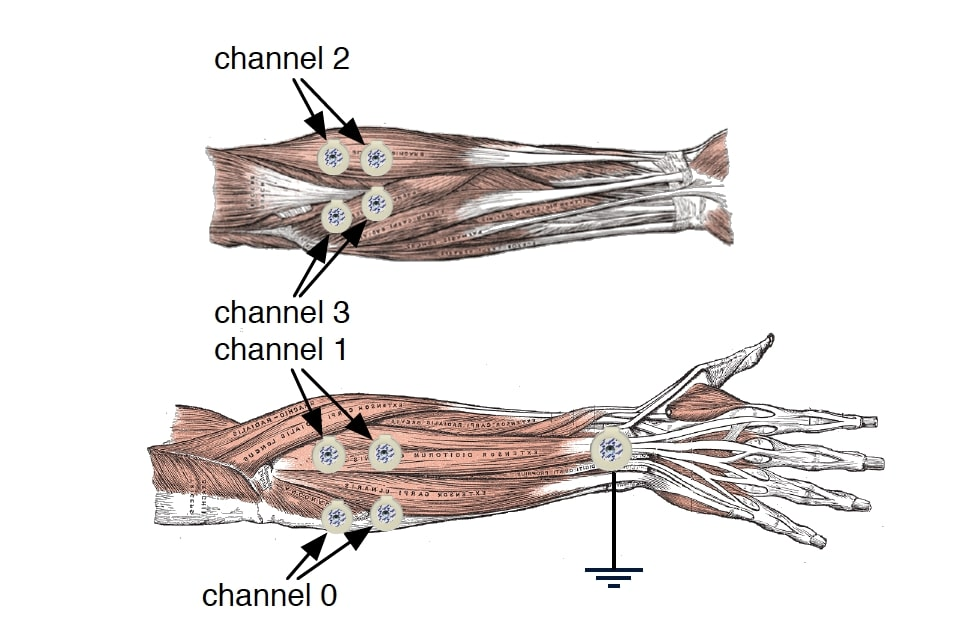
\includegraphics[scale=0.17]{grafiken/electrode-positioning.jpg}
	\caption{Position der Elektroden am Unterarm (\cite{Kaufmann2013Data})}
	\label{elektroden-position}
	\end{center}
\end{figure}
% Allgemeine Eigenschaften des Datensatzes (Zeitraum, Frequenz, Beschaffenheit der Daten)
Für das Erfassen der Daten wurde dem Proband im Rahmen der Forschung durch \cite{Kaufmann2013Data} ein tragbares Datenerfassungssystem mit vier EMG-Kanälen am Unterarm angelegt (Abbildung \ref{elektroden-position}). Dieses zeichnete die elektrischen Signale mit einer Auflösung von 24 bit und einer sampling rate von 2048 Hz auf. Dabei wurde die Position der Elektroden nach der ersten Aufzeichnung auf der Haut des Probanden markiert, um in folgenden Aufzeichnungen die Position replizieren zu können und so Ungenauigkeiten bei der Messung einzugrenzen. 

In jeder Aufnahmesitzung wurden mehrere Bewegungen in Folge erfasst. Jede Bewegung besteht dabei aus einer vier-sekündigen Entspannungs- und einer fünf-sekündigen Kontraktionsphase. Die Kontraktionsphase lässt sich dabei wiederum in eine ein-sekündige Anfangsphase und eine vier-sekündige stetige Phase unterteilen (\cite{Kaufmann2013Data}). 


\begin{figure}[h]
	\begin{center}
	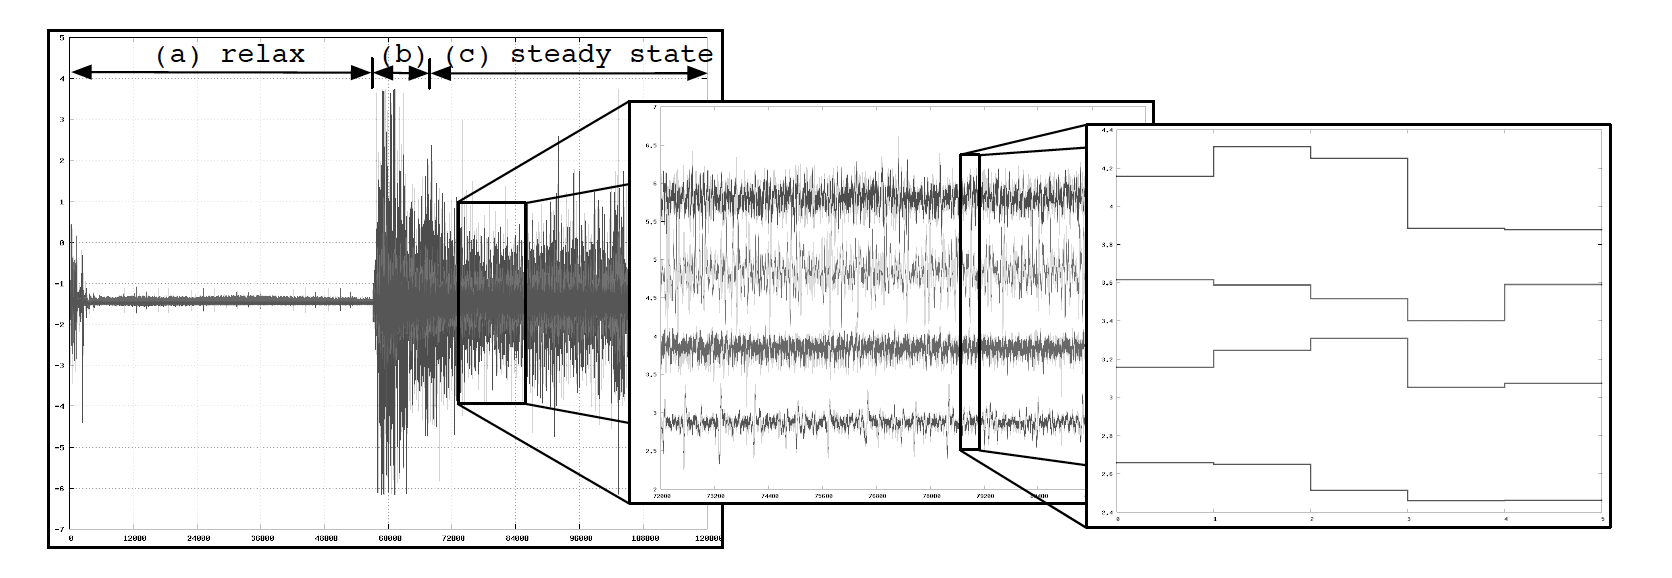
\includegraphics[scale=0.4]{grafiken/feature-extraction.png}
	\caption{Merkmalsextraktion aus der stetigen Phase (\cite{Kaufmann2013Data})}
	\label{feature-extraction}
	\end{center}
\end{figure}

Wie in Abbildung \ref{feature-extraction} zu sehen ist, erfolgte die Merkmalsextraktion anhand des Signals in der stetigen Phase.
Dieser Abschnitt wird in Fenster von jeweils 150ms unterteilt, aus denen jeweils die Merkmale extrahiert werden. Anschließend wird das Fenster um 150ms verschoben. Auf diese Weise bleiben die Aufzeichnungen der Klassen untereinander differenzierbar und das Signal wird gleichzeitig um überschüssiges Rauschen bereinigt, um die rechnerische Intensität zu verringern (\cite{Kaufmann2013Data}). 


\begin{figure}[ht]
	\begin{center}
	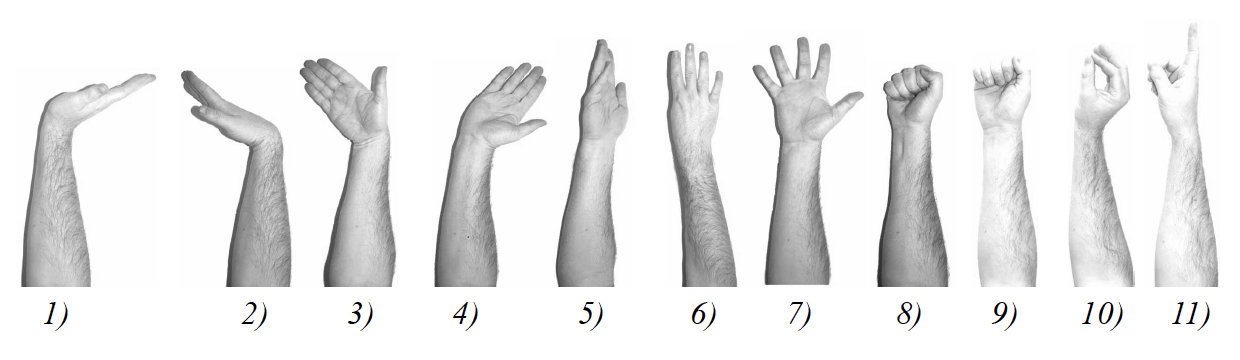
\includegraphics[scale=0.5]{grafiken/11classes.png}
	\caption{Im Datensatz enthaltene Merkmale (\cite{Kaufmann2013Data})}
	\label{bewegungsklassen}
	\end{center}
\end{figure}


% Kurze Vorstellung der Merkmale
Der Datensatz enthält laut \cite{Kaufmann2013Data}, wie in Abbildung \ref{bewegungsklassen} zu sehen, elf gekennzeichnete Bewegungen des Handgelenks, die alle jeweils über den gesamten Aufzeichnungszeitraum erfasst wurden. Enthalten ist 1) die Streckung, 2) die Beugung, 3) die Ulnare Abduktion, 4) die Radiale Abduktion, 5) die Innenrotation, 6) die Außenrotation, 7) das Öffnen, 8) das Schließen, 9) der Schlüsselgriff, 10) der ''Pincher-Grip'' und 11) das Ausstrecken des Zeigefingers.

\section{Extrahierte Merkmale}

% Detaillierteres Eingehen auf die aus dem Zeitbereich extrahierten Merkmale
Aus den vier je Elektrode extrahierten Merkmalen entsteht somit eine Liste aus $4 * 4 = 16$ Merkmalen für jedes Fenster in der jeweiligen Aufzeichnung (\cite{Kaufmann2013Data}). Es handelt sich wie bereits im vorigen Kapiteln erwähnt um Merkmale aus dem Zeitbereich, die bereits in dem Papier von \cite{zecca2002control} detailliert beschrieben wurden und auf die nun im Folgenden weiter eingegangen wird.

Nach \cite{Engelhart2003} setzen sich die extrahierten Klassen wie folgt zusammen:

\textit{Mean Absolute Value (MAV)}:
Der Mean Absolute Value bildet den Durchschnittswert eines Signals $x$ über den Zeitraum $i$, der in Summe $L$ Signale enthält.

$$\bar{x}_i = \frac{1}{L}\sum_{k=1}^{L}|x_k|\;f\ddot{u}r\;i=1,...,I$$

\textit{zero crossings (ZC)}:
Zero Crossings geben an, wie häufig ein Signal die Nullmarke passiert. Um durch Rauschen ausgelöste Überschreitungen auszuschließen, wird dafür eine Schwelle $\varepsilon$ festgelegt. Vergleicht man also nun die zwei Punkte $x_k$ und $x_k+1$ im Verlauf des Signals, kann man die Anzahl der Nulldurchgänge um 1 erhöhen, wenn folgende Bedingungen gegeben sind:

$$\{x_k > 0 \;und\; x_{k+1} < 0\}\;oder\;\{x_k < 0\;und\;x_{k+1} > 0\}$$
$$|x_k - x_{k + 1}| \geq \varepsilon$$


\textit{slope sign changes (SSC)}:
Die Anzahl der slope sign changes, also der Vorzeichenwechsel der Steigung in einem aufgezeichneten Signal, werden ebenfalls als Merkmal verwendet. Sie funktionieren dahingehend ähnlich wie ZC, da hier ebenfalls jedes Mal, wenn ein aufgezeichnetes Signal die Schwelle $\varepsilon$ überschreitet, ein Zähler inkrementiert wird. Betrachtet werden dabei auf dem Signal die Punkte $x_{k - 1}$, $x_k$ und $x_{k+1}$. Inkrementiert wird unter folgenden Bedingungen:

$$\{x_k > x_{k-1}\;und\;x_k > x_{k+1}\}\;oder\;\{x_k < x_{k-1}\;und\;x_k<x_{k+1}\}$$
$$|x_k-x_{k+1}|\geq\varepsilon\;oder\;|x_k-x_{k-1}|\geq\varepsilon$$

\textit{waveform length (WL)}:
Die durch die nachfolgende Formel von \cite{Engelhart2003} beschriebene waveform length gibt die Signallänge des jeweiligen Aufnahmefensters an. Diese ergibt sich aus der kummulierten Differenz $\Delta{x_k}$ der Punkte $x_k$ und $x_{k-1}$ über die gesamte Summe der Signale L (\cite{Engelhart2003}).

$$l_0=\sum_{k=1}^{L}|\Delta{x_k}|$$

Nach erfolgter Extraktion werden die 16 erfassten Merkmale pro Zeitfenster zu einer Liste zusammengefügt. Das 17te Element der Liste kodiert dabei die in diesem Fenster aufgenommene Klasse, während das 18te Element die Aufnahmesitzung angibt. Dadurch entsteht eine Liste aus mit der jeweiligen Klasse und der Aufnahmesitzung kodierten Merkmalen (Abbildung \ref{dataset-item}), mit denen nun die Klassifikatoren trainiert werden können.
\bigskip
\begin{figure}[h]
	\begin{center}
		\begin{tikzpicture}[scale=0.8]
		\draw[black, thin] (0,0) rectangle (3,1);
		\draw[decoration={brace,mirror,raise=5pt},decorate]
		(0+0.1,0) -- node[below=6pt] {Elektrode 1} (3-0.1,0);
		
		\draw[black, thin] (3,0) rectangle (6,1);
		\draw[decoration={brace,mirror,raise=5pt},decorate]
		(3+0.1,0) -- node[below=6pt] {Elektrode 2} (6-0.1,0);
		
		\draw[black, thin] (6,0) rectangle (9,1);
		\draw[decoration={brace,mirror,raise=5pt},decorate]
		(6+0.1,0) -- node[below=6pt] {Elektrode 3} (9-0.1,0);
		
		\draw[black, thin] (9,0) rectangle (12,1);
		\draw[decoration={brace,mirror,raise=5pt},decorate]
		(9+0.1,0) -- node[below=6pt] {Elektrode 4} (12-0.1,0);
		
		\draw[black] (12,0) rectangle (13.5,1);
		\draw[black] (13.5,0) rectangle (15,1);

		\node at (0+1.5,0+0.4) {$m_{11}$, ..., $m_{14}$};
		\node at (3+1.5,0+0.4) {$m_{21}$, ..., $m_{24}$};
		\node at (6+1.5,0+0.4) {$m_{31}$, ..., $m_{34}$};
		\node at (9+1.5,0+0.4) {$m_{41}$, ..., $m_{44}$};
		\node at (12+0.75,0+0.45) {k};
		\node at (13.5+0.75,0+0.45) {t};
		\end{tikzpicture}
		\caption{Aufbau eines Eintrags im Datensatz, während $m_{1x}$ das $x$te Merkmal der 1. Elektrode bezeichnet. Die aufgezeichnete Klasse wird durch $k$ und die aktuelle Aufnahmesitzung durch $t$ gekennzeichnet (eigene Darstellung).}
		\label{dataset-item}
	\end{center}
\end{figure}


\chapter{Einführung Tiefe Neuronal Netze}
\label{chap:dnn}

Die folgenden Abschnitte beschreiben die Funktionsweise von Neuronalen Netzen auf Basis der Erläuterungen in \cite{haykin2007neural}. Neuronale Netze sollen nach \cite{haykin2007neural} in ihrer ursprünglichen Form die neuralen Strukturen des menschlichen Gehirns abbilden. Sie sollen, anders als beispielsweise konventionelle Computer, über die Möglichkeit verfügen, zu lernen. Parallelen zwischen Neuronalen Netzen und menschlichen aus Synapsen bestehenden Strukturen im Gehin sind nach \cite{haykin2007neural}:

\begin{enumerate}
    \item \glqq Das Akquirieren von Wissen des Netzwerks durch einen von der Umgebung\linebreak abhängigen Lernprozess\grqq{} (\cite{haykin2007neural})
    \item \glqq Die Stärke von Interneuronalen Verbindungen, bekannt als synaptische Gewichte, wird verwendet um akquirierte Informationen zu speichern\grqq{} (\cite{haykin2007neural})
\end{enumerate}

\cite{haykin2007neural} beschreibt Neuronale Netze dabei als Netzwerke aus Schichten, die wiederum aus einzelnen Neuronen bestehen. Diese Neuronen sind von Schicht zu Schicht miteinander verbunden. Solche Verbindungen ähneln wie von \cite{haykin2007neural} ursprünglich beschrieben Synapsen mit Gewichten, durch die das Netzwerk lernt, welche Verbindungen mehr und welche weniger \glqq gestärkt \grqq{} werden müssen, um ein richtiges Ergebnis zu erhalten. So eine Verbindung $i$ setzt sich in einem Neuronalen Netz also vereinfacht stets zusammen aus Gewicht $w$, dem Input-Signal des eingebenden Neurons $y$ und dem Bias $b$.

$$i=w*y-b$$

Ein Neuron besteht somit nach \cite{haykin2007neural} aus der Summe aller seiner einfließenden Verbindungen. Die einfachste Form eines Neuralen Netzes ist demnach ein \textit{Single-Layer Feedforward Network} mit nur einer Schicht, welches auch allgemein als Perzeptron bezeichnet wird. Fügt man eine Schicht zwischen dem Input- und Output-Layer hinzu, so bezeichnet man diese als \textit{hidden layer} (HL). Hidden Layer dienen nach \cite{haykin2007neural} dazu, den Input des Netzwerks vor der Ausgabe zu verarbeiten, wodurch das Netzwerk komplexere Aufgabenstellungen lösen kann. Solche Netzwerke benötigen laut \cite{haykin2007neural}, um nicht auf die Input-Output Beziehung eines gewöhnlichen Perzeptrons reduziert zu werden, sogenannte nicht-lineare Aktivierungsfunktionen. Eine häufig verwendete Aktivierungsfunktion ist hier laut \cite{haykin2007neural} die \textit{Sigmoid}-Aktivierungsfunktion, wobei die \textit{Rectified Linear Unit}-Aktivierungsfunktion besonders in den letzten Jahren an Beliebtheit gewann (\cite{lecun2015deep}), was auf ihre guten Ergebnisse (\cite{nair2010rectified}), sowie bessere Kompatibilität mit besonders Tiefen Neuronalen Netzen aufgrund von Effekten wie dem \textit{Vanishing Gradient} (\cite{hochreiter2001gradient}) zurückzuführen ist. Ein solches Neuron setzt sich also im Fall von $n$ einfließenden Verbindungen vereinfacht wie folgt zusammen:

$$i=\sigma(w_1y_1+w_2y_2+w_3y_3+...+w_na_n - b)$$

$\sigma$ steht dabei in diesem Fall für die \textit{Sigmoid}-Aktivierungsfunktion. Netzwerke mit mehr als zwei Schichten, also mindestens zwei HL und einem Output Layer, werden als Tiefe Neuronale Netze bezeichnet. Netzwerke lernen laut \cite{haykin2007neural} durch schrittweise Korrektur von Fehlern in den Gewichten des Netzwerks. Das geschieht mittels dem \textit{Backpropagation} (BP) Algorithmus. Das Netzwerk wird dabei einmal vorwärts mit statischen Gewichten und rückwärts mit Anpassung der Gewichte durchlaufen. Dabei wird am Ende des ersten Durchlaufes nach vorne der Fehlerwert für jedes Output-Neuron bestimmt. Die quadrierte Summe aller Fehler der Neuronen ergibt die \textit{Kostenfunktion} des Netzwerks. Anschließend wird ein \textit{Gradient} berechnet, der die Richtung und Intensität der Anpassung im Gewichts des Neurons angibt. Diese Anpassung wird als \textit{Gradientenabstieg} bezeichnet und hat als Ziel, die Kostenfunktion des Netzwerks zu minimieren. Der Gradient kann nun mit der Lernrate, die als Hyperparameter festgelegt werden kann und damit die Größe der getätigten Schritte Richtung Optimum kontrolliert, und dem Input-Signal des Neuronen multipliziert werden, um die vorzunehmende Korrektur des Gewichts zu erhalten. Eine solche Optimierung der Kostenfunktion kann so rekursiv rückwärts auf jede Schicht in dem Netzwerk angewandt werden, um sich schrittweise einem Optimum zu nähern (\cite{haykin2007neural}).

Tiefe Neuronale Netze sind unter anderem deshalb Schwerpunkt dieser Arbeit, da diese in der Forschung zu der Klassifikation von EMG Signalen bereits gute Ergebnisse erzielten. So wurden in der Vergangenheit bereits Convolutional Neural Networks in Verbindung mit EMG-Datensätzen trainiert und erzielten sowohl mit konventionell initialisierten Gewichten (\cite{Allard2019}, \cite{geng2016gesture}), als auch mit durch Techniken des \textit{Transferlernens} initialisierten Gewichten, also mit Gewichten, die bereits durch die selbe oder andere Architekturen vortrainiert wurden, präzise Klassifikationsgenauigkeiten (\cite{cote2017transfer}). Auch in dem in dieser Arbeit weiter beleuchteten Bereich der \textit{Recurrent Neural Networks} wurden in der Vergangenheit für die Klassifikation von EMG Signalen bereits durch \cite{simao2019emg}, \cite{bu2003emg} und \cite{tsuji2000pattern} gute Ergebnisse in der Klassifikation erzielt.
\chapter{Experimenteller Aufbau}
\label{chap:experiment}

Als Kern dieser Arbeit werden sowohl die RNN-Architekturen gewöhnliche RNN, LSTM und GRU, als auch die klassischen Klassifikatoren kNN, SVM, MLP und DT implementiert, getestet, ausgewertet und miteinander verglichen. Das Experiment verwendet, um Vergleichbarkeit sicherzustellen, für alle Klassifikatoren denselben in Kapitel 3 beschriebenen \glqq 121 Forearm EMG\grqq{} Datensatz von \cite{Kaufmann2013Data}. Um eine möglichst hohe Generalisierbarkeit der erzielten Ergebnisse zu erreichen, wurden alle Architekturen mittels einer 10-fachen \textit{Cross Validation} evaluiert. Diese ist nach \cite{kohavi1995study} ein Vorgehen zum Sicherstellen der Generalisierbarkeit von Ergebnissen und geschieht durch die Aufteilung des Datensatzes in $k$ inetwa gleich große Abschnitte. Daraufhin wird der Klassifikator einmal mit jedem Abschnitt der Daten getestet und mit dem Rest trainiert. Daraus ergibt sich eine durchschnittliche Klassifikationsgenauigkeit aus allen $k$ Durchläufen und vermeidet dadurch, dass manche Klassifikatoren durch zufällig \glqq einfacher\grqq{} zu klassifizierende Daten besser abschneiden. Gleichzeitig bedeutet k-fache Cross Validation aber auch einen dementsprechend höheren rechnerischen Aufwand (\cite{kohavi1995study}). Alle Hyperparameter werden aufgrund der rechenintensiven Natur mancher Klassifikatoren manuell optimiert. Im Fall der RNN-Architekturen wurde eine Lernrate von 0,001 gewählt. Um Overfitting in den RNN-Architekturen zu Vermeiden, wurde in diesen die \textit{Dropout}-Methodik (\cite{srivastava2014dropout}) verwendet. Diese schließt während des Trainings zufällig einen gewissen Prozentteil der Neuronen, inklusive ihrer Verbindungen, aus (\cite{srivastava2014dropout}). Dadurch passen sich Neuronen weniger aufeinander an und das Potenzial für Overfitting wird nach (\cite{srivastava2014dropout}) reduziert (\cite{srivastava2014dropout}). Um \textit{internal Covariance Shift} zu vermeiden, der durch die Anpassung der Gewichte und die dadurch entstehenden Unterschiede in der Verteilung der Neuronen in DNN zu Problemen führen kann (\cite{ioffe2015batch}), wird für das Training der RNN Strukturen \textit{Batch Normalization} (\cite{ioffe2015batch}) verwendet. Die Konfiguration sowie das Training und die Auswertung der verschiedenen Klassifikatoren geschieht mithilfe der Keras API von Tensorflow und Scikit Learn in der Programmiersprache Python. Das Training erfolgt in der CPU-Version von Tensorflow auf einem Intel 2,3 GHz 8-Kern i9 Prozessor.

Primäre Metriken für den Vergleich der Klassifikatoren sind die Klassifikationsgenauigkeit sowie die Trainingsdauer. Zunächst werden die gewöhnlichen state-of-the-art Klassifikatoren kNN, SVM, MLP und DT miteinander verglichen und potenzielle Besonderheiten in der Auswertung dieser aufgeführt. Anschließend werden die RNN-Architekturen zunächst miteinander und anschließend mit den am besten abschneidenden state-of-the-art Klassifikator verglichen, wobei hier ebenfalls auf Besonderheiten in den Ergebnissen und der Auswertung hingewiesen wird. Die Vorstellung und Auswertung der Ergebnisse erfolgt in Kapitel 8.
\chapter{Recurrent Neural Networks}
\label{chap:rnn}
Ein Schwerpunkt dieser Arbeit sind RNN. Diese speziell für die Klassifikation und Regression von sequentiellen Daten entwickelte DNN-Architektur findet besonders in Anwendungsfällen, in denen die Reihenfolge von Daten eine dominante Rolle in der Richtigkeit der Klassifikation spielt, Verwendung. Auch im Bereich der Klassifikation von sEMG-Signalen wurden RNN in der Vergangenheit bereits erfolgreich utilisiert (\cite{simao2019emg}). Trotz der Möglichkeit der Interpretation von sequentiellen Daten ergeben sich bei der Arbeit mit RNN einige Schwierigkeiten (\cite{pascanu2013difficulty}), weshalb das Training solcher Netzwerke nicht immer problemlos verläuft. Insbesondere die \textit{Vanishing Gradient} (VG) und \textit{Exploding Gradient} (EG) Problematiken sind nach \cite{pascanu2013difficulty} typisch und werden im Folgenden ebenfalls beschrieben. Um diese zu umgehen, werden in dieser Arbeit zusätzlich \textit{long short term memory} und \textit{gated recurrent unit} Architekturen verwendet und ebenfalls weiter ausgeführt.

\section{Einführung Recurrent Neural Networks}
\label{sec:rnn}
RNN ähneln nach \cite{pascanu2013difficulty} in ihrer Architektur gewöhnlichen MLP. Im Fall von RNN werden die HL jedoch rekurrent durchlaufen, um aus Sequenzen zu lernen. Das bedeutet, dass ein HL für jeden Input in einer Sequenz einmal durchlaufen wird und der Output des vorherigen Durchlaufs stets zum Input des nächsten Durchlaufs hinzugefügt wird. 

\begin{figure}[h]
    \begin{center}
        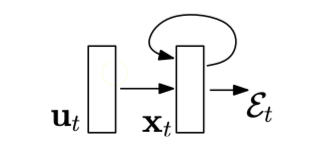
\includegraphics[scale=0.8]{grafiken/rnn-basic.png}
        \caption{Grundlegender Aufbau eines RNN mit Input Layer $u_t$ und HL $x_t$ (\cite{pascanu2013difficulty})}
        \label{rnn-basic}
    \end{center}
\end{figure}

Durch diesen Aufbau können RNN theoretisch Sequenzen beliebiger Länge durchlaufen und diese erlernen (\cite{pascanu2013difficulty}). 

% Mathematischer Aufbau hinzufügen

Um das Training von RNN mit dem aufgezeichneten Datensatz zu ermöglichen, wurden die darin enthaltenen Daten in solche Sequenzen unterteilt. Da es sich hier um ein Problem der Klassifikation handelt und jede Sequenz von Daten einem Ergebnis entspricht, wurden die im Datensatz enthaltenen Aufnahmen für diese Arbeit nach aufeinanderfolgenden Bewegungsklassen gruppiert. Die daraus entstehenden Sequenzen wurden mit der jeweils zugehörigen Klasse gelabelt und anschließend in die Architekturen hineingegeben.

Zunächst wurde ein gewöhnliches RNN untersucht. Hierfür wurde nach händischer Optimierung eine Struktur mit vier HL gewählt. Die ersten drei HL mit je 124 Neuronen waren dabei RNN Schichten, die jeweils die Sequenzen rekurrent durchliefen, bevor die Daten an die vierte Schicht, einen Dense-Layer mit 32 Neuronen und einer Rectifier Linear Unit (ReLU) Aktivierungsfunktion, übergeben wurden. Dieser übergab die Daten an den Output Layer mit elf Neuronen, der nach Durchlaufen einer Softmax Aktivierungsfunktion das Ergebnis der Klassifikation ausgab. Diese Architektur wurde über 100 Epochen mit dem Datensatz trainiert und mittels zehnfacher Cross Validation evaluiert.

Unter der Betrachtung der erzielten Klassifikationsgenauigkeit auf dem Validierungsdatensatz waren die Ergebnisse dieser Architektur zunächst vergleichbar mit der Genauigkeit anderer Klassifikatoren wie dem MLP oder kNN.
So stellte sich nach der 47. Epoche eine Asymptotisierung ein und die Genauigkeit der Klassifikation schwankte nur noch um die 85\% Marke. Dies kann man an Abbildung \ref{srnn-1-acc} erkennen.

\begin{figure}[h]
    \begin{center}
        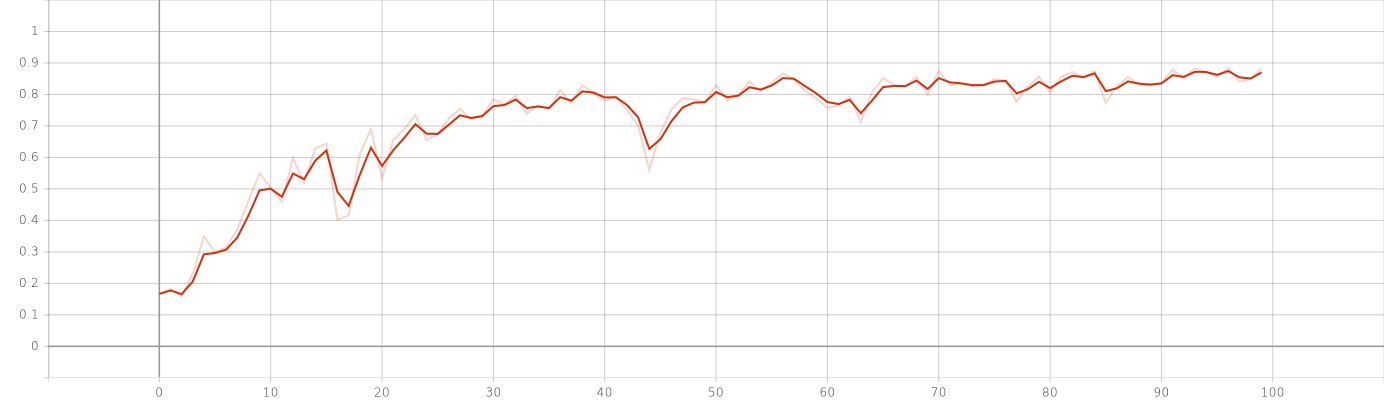
\includegraphics[scale=0.3]{grafiken/srnn-1-acc.png}
        \caption{Darstellung der Genauigkeit auf dem Validierungsdatensatz in Abhängigkeit der Epoche}
        \label{srnn-1-acc}
    \end{center}
\end{figure}

Das untersuchte Netzwerk unterliegt hier allerdings noch einigen Einbußen, die durch Betrachten der Entwicklung des Klassifikationsfehlers in Abhängigkeit der Epoche auffallen. Während diese nämlich im Fall von gewöhnlich lernenden Netzwerken stetig fallen sollte, enthält die Grafik der untersuchten Netzwerkarchitektur große Ausschläge im Verlauf des Trainings (Abbildung \ref{rnn-1-loss}).

\begin{figure}[h]
    \begin{center}
        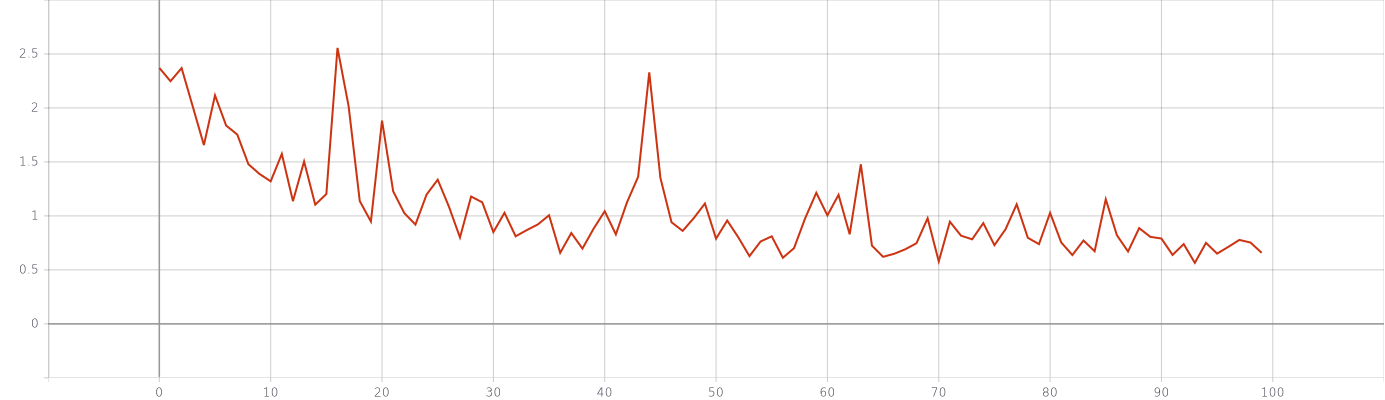
\includegraphics[scale=0.3]{grafiken/rnn-1-loss.png}
        \caption{Klassifikationsfehler der RNN Architektur in Abhängigkeit der Epoche}
        \label{rnn-1-loss}
    \end{center}
\end{figure}

Diese starken Ausschläge im Fehlerwert der Klassifikation deuten nach \cite{pascanu2013difficulty} häufig auf die Problematik eines \textit{Exploding Gradient} hin. Diese entsteht im Kontext von RNN-Architekturen während der Gradientenberechnung in der \textit{Backpropagation Through Time} (BTT) (\cite{werbos1990backpropagation}). Da Neuronale Netze wie in Kapitel 4 dieser Arbeit Informationen durch die Gewichtung einzelner Neuronen speichern (\cite{haykin2007neural}), wird dieser Mechanismus auch in RNN genutzt um Informationen vorheriger Durchläufe der Sequenzen zu speichern (\cite{werbos1990backpropagation}). Somit betrifft BTT nicht nur die Anpassung der Parameter von Layer zu Layer, sondern auch von Sequenzabschnitt zu Sequenzabschnitt (\cite{werbos1990backpropagation}). So wird zur Initialisierung eines Neurons in einem RNN stets der \textit{hidden state} des vorherigen Durchlaufs hinzugefügt und so forwärtspropagiert (\cite{pascanu2013difficulty}). Vor allem bei langen Sequenzen, in denen die Gewichte der Aktivierungsfunktion $w > 1$ entsprechen, kommt es durch die mehrfache Multiplikation der Werte zu sehr hohen Gradientenwerten gegen unendlich, die das Netzwerk mit einem Durchlauf bereits sehr stark beeinflussen. EG sind zwar kein Problem, das sich auf RNN beschränkt, sie sind hier allerdings aufgrund der in diesen angewandten BTT in solchen Architekturen häufiger anzutreffen (\cite{pascanu2013difficulty}).

Eine von \cite{pascanu2013difficulty} angesprochene und in der Praxis häufig angewandte Methode ist die des \textit{gradient clipping} (GC). Hier wird für den Gradienten eine Schwelle festgelegt, auf die er reduziert oder erhöht wird, sollte er diese über- oder unterschreiten. Das begrenzt den Gradienten auf einen bestimmten Wertebereich und unterbindet somit die für EG üblichen starken Ausschläge. Die Verwendung von GC in der untersuchten Architektur führte zu einer mit weniger Ausschlägen verlaufenden Fehler- und Klassifikationsgenauigkeitskurve.

GC glättet zwar den Verlauf des Klassifizierungsfehlers und macht diesen insgesamt weniger volatil, reduziert allerdings ebenfalls die erzielte Klassifizierungsgenauigkeit der Architektur. Während dies aufgrund des stagnierenden Fehlerwertes und somit potenziell stagnierenden Gewichten auf den gegenteiligen Effekt des GC, den \textit{vanishing gradient} (VG), hinweisen könnte, ist das Nachweisen von VG in RNN anhand der vorhandenen Daten schwierig. Um die Schwierigkeiten rund um EG und VG zu umgehen, können die RNN-Architekturen LSTM und GRU verwendet werden (\cite{simao2019emg}), die im Verlauf dieser Arbeit ebenfalls auf den Datensatz angewandt wurden und gute Ergebnisse erzielten.

Zwar erreichte die gewöhnliche RNN-Architektur nach Optimierung und Einsatz von GC eine stabile Klassifikationsgenauigkeit, sie führte allerdings im Hinblick auf die Trainingsdauer und den Vergleich mit einfacheren Klassifikatoren wie dem MLP, kNN oder SVM zu Ergebnissen, die eine praktische Anwendung der Architektur ausschließen würden. Andere Klassifikatoren erreichten hier in einer häufig geringeren Trainingsdauer präzisere Klassifikationsergebnisse, wie in Kapitel 7 dieser Arbeit aufgezeigt wird.


\section{Long Short Term Memory}
\label{sec:lstm}

Während RNN auf gewöhnlichen Feed-Forward-Netzen aufbauen, in dem sie die HL mit Schleifen versehen und dadurch die zeitlichen Beziehungen interpretieren können (\cite{simao2019emg}), haben gewöhnliche RNN Strukturen häufig Probleme bei Sequenzen mit langer Aufnahmespanne (\cite{pascanu2013difficulty}). Typische Konsequenzen sind hier wie obig angesprochen die VG- und EG-Problematik. LSTM-Architekturen lösen dieses Problem, indem sie die Anzahl der Gewichte und Biases eines in einem RNN enthaltenen Neurons vervierfachen. Dadurch erhält das Netzwerk die Möglichkeit, vergangene Informationen durch sogenannte Gates zu filtern (\cite{simao2019emg}). Diese Kombinationen aus Gewicht und Bias ergeben nach \cite{simao2019emg} folgende Gates:

\begin{itemize}
    \item \textit{input gate layer} (IGL)
    \item \textit{forget gate layer} (FGL)
    \item \textit{output gate layer} (OGL)
    \item \textit{state gate layer} (SGL)
\end{itemize}

Der FGL und IGL bestimmen durch ihr Gewicht und Bias, wie der \textit{hidden state} der letzten Sequenz und der aktuelle Input die Aktivierung des aktuellen Neurons beeinflussen. Die nachfolgenden von \cite{simao2019emg} aufgestellten Gleichungen zeigen dies mathematisch auf.

$$i_t=\sigma(W_i*[h_{t-1}, x_t]+b_i)$$
$$f_t=\sigma(W_f*[h_{t-1}, x_t]+b_f)$$

Dabei stellen die mit $i$ indexierten Gewichte und der Bias die trainierbaren Parameter des IGL und die mit $f$ indexierten Parameter die des FGL dar. $t$ steht für die aktuelle zeitliche Sequenz (\cite{simao2019emg}). 

Diese zwei Sigmoid Funktionen ergeben Werte zwischen 0 und 1, die durch Multiplikation mit dem \textit{cell state} (CS) der vorgehenden Periode $c_{t-1}$ und dem vorläufigen CS der neuen Periode $\widetilde{c}_t$ jeweils den Einfluss auf den CS der aktuellen Period $c_t$ steuern. $\widetilde{c}_t$ entspricht dabei, wie in der folgenden Gleichung zu sehen, dem CS eines normalen RNN. Der Einfluss von diesem auf den neuen CS wird hier allerdings durch den IGL geregelt.

$$\widetilde{c}_t=tanh(W_c*[h_{t-1}, x_t]-b_c)$$

Der zum Schluss ausgegebene CS setzt sich somit zusammen aus dem CS der vorigen Periode $c_{t-1}$ und dem vorläufigen CS $\widetilde{c}_t$ der aktuellen Periode, gewichtet mit dem Wert des VGL und des IGL.

$$c_t=f_t*c_{t-1}+i_t*\widetilde{c}_t$$

Durch den OGL wird der an den nächsten Schritt übergebene \textit{hidden state} (HS) gesteuert. So ergibt sich der weitergegebene HS $h_t$ aus dem Ergebnis der OGL $o_t$ multipliziert mit durch die tang-Aktivierungsfunktion normierte CS $c_t$.

$$o_t=\sigma(W_o*[h_{t-1}, x_t]-b_o)$$
$$h_t=o_t*tanh(c_t)$$

Durch diese Gates kann der CS und HS auch über lange Sequenzen hinweg erhalten bleiben. Das führt dazu, dass das Netzwerk lange zurückliegende Abschnitte von Sequenzen nicht vergisst, sondern beibehält und dadurch die Problematiken des VG und EG in gewöhnlichen RNN löst (\cite{simao2019emg}). 

Auch unter Training auf dem in dieser Arbeit verwendeten Datensatz erzielte die LSTM Architektur gute Ergebnisse. Insbesondere im Vergleich mit gewöhnlichen RNN fällt die starke Erhöhung in der Klassifikationsgenauigkeit auf dem Validierungsdatensatz und die schnelle Asymptotisierung desselbigen auf. Auch die Volatilität sowohl des Klassifikationsfehlers als auch der Klassifikationsgenauigkeit in Abhängigkeit der Epoche reduzierte sich, wie in den Abbildungen \ref{lstm-acc} zu sehen, drastisch. Die LSTM-Architektur erzielte nach 100 Epochen eine Klassifikationsgenauigkeit von 98,11\%. Anzumerken ist hierbei allerdings, dass hierfür eine Trainingsdauer von 58 Minuten und 28 Sekunden benötigt wurde, was der höchsten in dieser Forschungsarbeit untersuchten Trainingsdauer entspricht.

\begin{figure}[h]
    \centering
    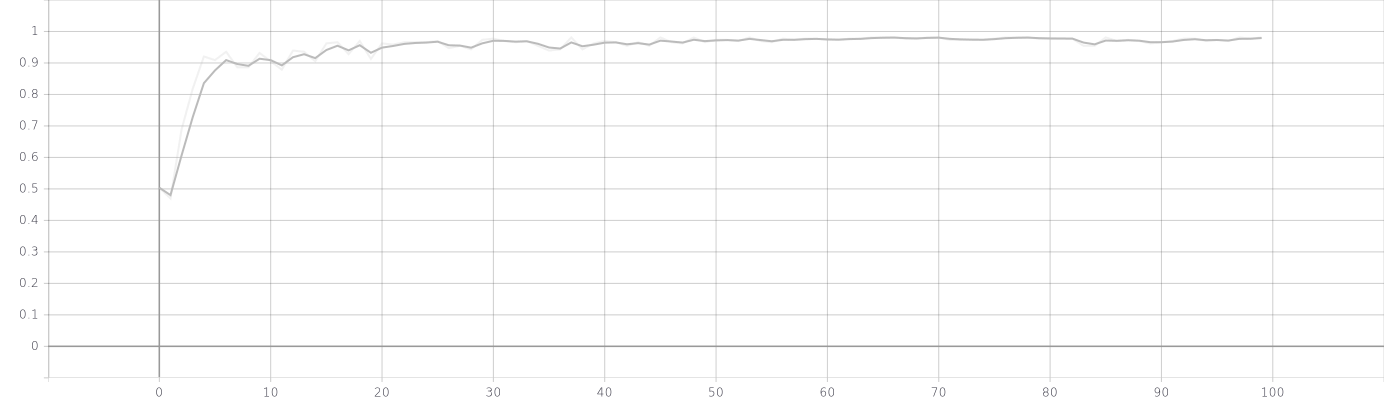
\includegraphics[scale=0.3]{grafiken/lstm-acc.png}
    \caption{Klassifikationsgenauigkeit der verwendeten LSTM Architektur in Abhängigkeit der Epoche auf dem Validierungsdatensatz}
    \label{lstm-acc}
\end{figure}


\section{Gated Recurrent Unit}
\label{sec:gru}

\textit{Gated Recurrent Units} (GRU) wurden durch \cite{cho-etal-2014-learning} mit derselben Intention entwickelt wie LSTM Architekturen und haben daher dieselben Vorteile gegenüber von gewöhnlichen RNN-Architekturen. Allerdings unterscheiden sich GRU in ihrer Funktionsweise und Parameteranzahl nach \cite{simao2019emg} von LSTM Architekturen. So ist ein Vorteil der GRU Architekturen gegenüber LSTM die reduzierte Parameterzahl. Diese führt zu einer schnelleren Trainings- und Klassifikationszeit (\cite{simao2019emg}). Die geringere Parameterzahl erreichen GRU durch eine geringere Anzahl an Gates. Anders als bei LSTM gibt es hier lediglich zwei mit trainierbaren Parametern. Diese sind das \textit{update gate} (UG) $z_t$ und das \textit{reset gate} (RG) $r_t$. Dies lässt sich durch folgende von \cite{simao2019emg} aufgestellten Gleichungen veranschaulichen:

$$z_t=\sigma(W_z*[h_{t-1}, x_t])$$ 
$$r_t=\sigma(W_r*[h_{t-1}, x_t])$$ 

Anders als im Fall von LSTM Architekturen enthalten GRU keinen CS, sondern vermitteln sämtliche sequentielle Daten über den \textit{hidden state} $h_t$ (\cite{simao2019emg}). Das RG bestimmt durch die Funktion von $\widetilde{h}_t$, wie viel der vorherigen Information nicht in den nächsten HS übergeben, also vergessen, werden soll. Dies geschieht durch die Gewichtung des vorigen HS $h_{t-1}$.

$$\widetilde{h}_t=tanh(W*[r_t*h_{t-1}, x_t])$$

Abschließend wird der ausgegebene HS $h_t$ berechnet, indem der vorige HS $h_{t-1}$ und der neue vorläufige HS $\widetilde{h}_t$ mithilfe von dem UG $z_t$ gewichtet werden.

$$h_t=(1-z_t)*h_{t-1}+z_t*\widetilde{h}_t$$

Wie an dem Aufbau der Funktionen von UG und RG zu erkennen, enthalten diese zusätzlich keinen Bias, was zu einer weiter reduzierten Zahl an trainierbaren Parametern beiträgt und somit die Trainings- und Klassifikationsdauer weiter verringert (\cite{simao2019emg}).

Auch in der im Zuge der Forschungsarbeit untersuchten GRU-Architektur ließ sich diese Annahme bestätigen. So ist die GRU Architektur mit einer Trainingsdauer von 18 Minuten und 2 Sekunden die schnellste DNN Architektur in diesem Experiment. Sie erreichte dabei mit einer 98,11\%igen Klassifikationsgenauigkeit dieselbe Präzision wie die LSTM Architektur in einem Drittel der Trainingsdauer.

\begin{figure}[h]
    \centering
    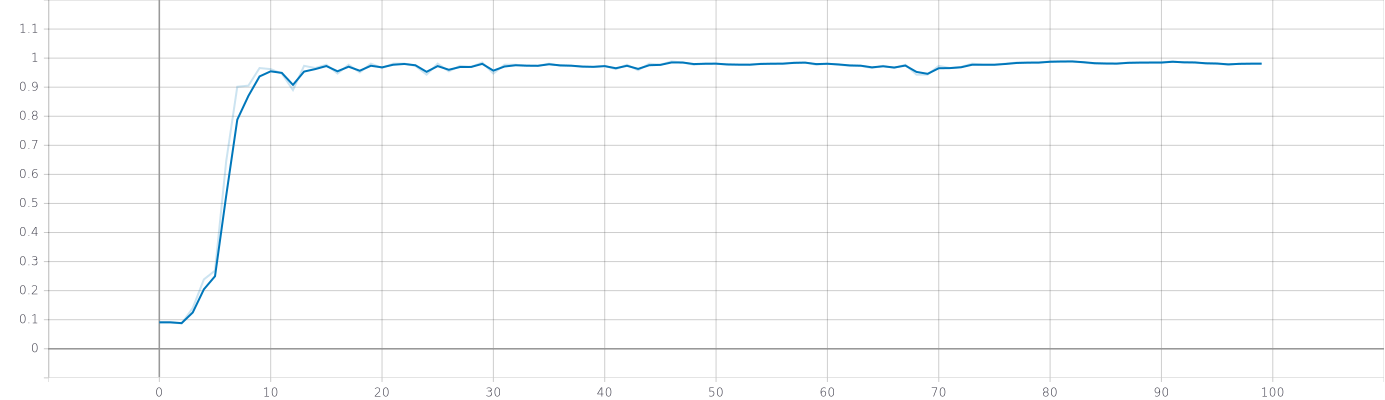
\includegraphics[scale=0.3]{grafiken/gru-acc.png}
    \caption{Klassifikationsgenauigkeit der GRU Architektur auf dem Validierungsdatensatz in Abhängigkeit der Epoche}
    \label{gru-acc}
\end{figure}
\chapter{Gewöhnliche Klassifikatoren}
\label{chap:other-classifiers}

Gegenstand dieser Arbeit ist der Vergleich einiger DNN, insbesondere im Bereich von RNN-Architekturen, mit anderen state-of-the-art Klassifikatoren. Namenhaft sind diese kNN, SVM, Entscheidungsbäume sowie als einziges verglichenes Neurales Netz ein MLP. In den folgenden Unterkapiteln werden die angesprochenen Klassifikatoren im Hinblick auf ihre Funktionsweise, Konfiguration und im Test mit dem Datensatz erzielten Ergebnissen dargestellt. Im folgenden Kapitel erfolgt anschließend die Auswertung und der Vergleich mit den behandelten RNN-Architekturen.


\section{k Nearest Neighbors}
\label{sec:knn}

kNN ist der simpelste in dieser Forschungsarbeit behandelte Algorithmus. Er beinhaltet nach \cite{Kaufmann2013} nur einen Parameter $k$, der für eine Klassifikation alle möglichen Werte durchlaufen muss, um den für den Datensatz besten Wert zu finden. Diese Eigenschaft sowie die zumeist im Vergleich zu anderen Klassifikatoren wie SVM, DT oder DNN geringere Klassifikationsgenauigkeit machen kNN zu einem Klassifikator, der in der Praxis selten Anwendung findet (\cite{Kaufmann2013}). Trotzdem wird er im Vergleich zu anderen Klassifikatoren gerne referenziert, so wie auch in dieser Arbeit. kNN benötigen nach \cite{Kaufmann2013} keine Trainingsphase. Es werden die $k$ nächsten Nachbarn des Wertes einer Klasse aus dem Trainingsdatensatz, gemessen nach Euklidischer Distanz, zum Setzen der Klassifikationsgrenze verwendet (\cite{Kaufmann2013}). Unter Verwendung dieser Abgrenzung wird anschließend der Validierungsdatensatz getestet und die Klassifikationsgenauigkeit bestimmt.

Mit einer Klassifikationsgenauigkeit von 82,92\% bei einem $k$ von 16 lieferte der kNN Algorithmus das für alle 17 durchlaufenen $k$s beste Ergebnis. Sowohl höhere, als auch niedrigere Werte für $k$ führen zu einer schlechteren Klassifikationsgenauigkeit.

\section{Support Vector Machines}
\label{sec:svm}

SVM verwenden nach \cite{duda2012pattern} sogenannte Kernel Funktionen, um systematisch Klassen in höheren Dimensionen, als der, in der die Daten vorliegen, zu separieren. \cite{duda2012pattern} spircht dabei von \glqq[der] Vorverarbeitung der Daten zum repräsentieren von Mustern in hohen Dimensionen\grqq{} \cite{duda2012pattern}. SCV sind dabei Hyperplanes mit einem sogenannten \textit{margin}, der den Astand zwischen den \textit{Support Vectros} (SV) und dem Hyperplane darstellt. Dabei gilt, dass die Klassifikationsgenauigkeit umso höher ist, je größer der Abstand zwischen den SV und dem Hyperplane ist. Diese einfache Variante der SVM bezeichnet man auch als \textit{Maximal Margin Classifier} (\cite{cristianini2000}). Diese sind in der Praxis nach \cite{cristianini2000} allerdings schlecht anwendbar, da sie keinen Klassifikationsfehler zulassen und somit entweder vorliegende Daten nicht klassifizieren können oder Overfitting eintritt. Aus diesem Grund wird ein sogenannter \textit{soft margin} (SM) verwendet, der anders als der in \textit{Maximal Margin Classifiers} verwendete \textit{margin}, Fehlklassifikationen zulässt, um auch in komplexen Anwendungen eine insgesamt höhere Klassifikationsgenauigkeit zu erreichen (\cite{cristianini2000}). Das entspricht dem Ansatz des \glqq Bias/Varianz Dilemmas\grqq{} in der Klassifikation von Daten nach \cite{friedman1997bias}, da hier durch Zulassen von Klassifikationsfehlern und somit einer geringeren Varianz, ein höherer Bias erzielt wird, der insgesamt zu einer besseren Klassifikationsgenauigkeit in Test-Datensätzen führt. SVM finden den optimalen Hyperplane rechnerisch effizient, ohne die Daten für den Vergleich vorerst in die jeweilige Dimension transformieren zu müssen (\cite{cristianini2000}). Dieses Vorgehen ist allgemein bekannt als der ''Kernel Trick''. Neben der rechnerischen Effizienz ist der größte Vorteil von SVM ihr unterliegendes Prinzip der Minimierung von Strukturiertem Risiko (\cite{Kaufmann2013}). Eine vergleichsweise gute Klassifikationsgenauigkeit des hier verwendeten Datensatzes ist somit zu erwarten, da MLP häufig gute Ergebnisse in der Generalisierung liefern (\cite{Kaufmann2013}).

Für diese Arbeit wurde die Lineare Kernel Funktion gewählt, da diese im Vergleich mit den anderen Kernel Funktionen mit 87,88\% die beste Klassifikationsgenauigkeit erzielte.

\section{Multi Layer Perceptron}
\label{sec:mlp}

MLP sind der einzige hier adressierte Klassifikator, der neben den RNN-Archtekturen aus der Domäne der Neuronalen Netze stammt. MLP besitzen mindestens zwei Schichten, also einen HL und eine Output-Schicht (\cite{jain1996artificial}). Sie nutzen für die Optimierung der Parameter BP, um durch Gradientenabstieg die Kostenfunktion des Netzwerkes zu minimieren (\cite{jain1996artificial}). Anders als Klassifizierer wie die SVM verfügen MLP nicht über Eigenschaften zur Minimierung von strukturiertem Risiko, weshalb mögliches Overfitting durch manuelles Testen und Anpassen der Hyperparameter, vermieden werden muss (\cite{Kaufmann2013}). Weiterhin muss die Struktur von MLP, genauso wie bei jedem Neuralen Netzwerk, über die Anzahl der Layer bishin zu Anzahl der Neuronen und der verwendeten Aktivierungsfunktionen händisch festgelegt und optimiert werden (\cite{haykin2007neural}).

Die im Rahmen dieser Forschung untersuchte MLP-Architektur wird, entsprechend der Anzahl an Merkmalen, durch einen Input Layer mit 16 Neuronen initialisiert. Anschließend werden die Daten an den HL mit 15 Neuronen und einer \textit{rectified linear unit} (ReLu) Aktivierungsfunktion initialisiert. Abschließend folgt der Output Layer mit elt, der Anzahl der Klassen entsprechenden, Neuronen und einer \textit{softmax} Aktivierungsfunktion, durch die eine der Klassen als Ergebnis des Durchlaufs ausgegeben wird. Das Modell verwendet den Adam Optimizer (\cite{kingma2014adam}) für die automatische Optimierung des \textit{Gradientenabstiegs} (GD) mit einer \textit{Lernrate} (LR) von 0.001 und einer \textit{Batch Size} (BZ) von 1054. Die Architektur wurde über 600 Epochen trainiert. Die Gewichte aller Layer wurden mit einer Gaußischen Normalverteilung, die Biases mit einer Konstante 0 initialisiert.

Die Architektur erreichte nach manueller Optimierung der Hyperparameter sowie der Struktur eine Klassifikationsgenauigkeit von 86,14\% nach einer Trainingsdauer von 3 Minuten und 42 Sekunden.

\section{Entscheidungsbäume}
\label{sec:decision-trees}

Nachfolgender Abschnitt beruft sich für die Beschreibung der Funktionsweise von Entscheidungsbäumen auf das Buch ''Pattern Classification'' von \cite{duda2012pattern}, welches sich mit verschiedenen Methoden der Klassifikation beschäftigt und den Aufbau von DT im Detail beschreibt. DT unterscheiden sich danach von den anderen hier untersuchten Klassifikatoren vor allem darin, dass anstatt der Verwendung von Vektoren und Zahlen zur Beschreibung und Klassifizierung von Mustern logisch angeordnete Listen von Eigenschaften verwendet werden. Sie benötigen daher für eine Klassifikation keine numerischen Daten, sondern können Muster auch anhand von mathematisch nicht greifbaren Konzepten wie beispielsweise Farben oder Geschmäckern unterscheiden. DT bilden eine baumartige Struktur aus sequentiellen ''ja/nein''- oder auch ''if/else''-Abfragen. Dabei ist die erste Abfrage, die sogenannte \textit{root node}, verbunden mit sukzessiven \textit{nodes}, die wiederum ''ja/nein''-Abfragen beinhalten (\cite{duda2012pattern}). Sogenannte \textit{leaf nodes} (LN), die keine anschließenden Verbindungen besitzen, stellen dabei eine Klassifizierungsentscheidung dar (\cite{Kaufmann2013}). Ein Vorteil dieser Architektur nach \cite{duda2012pattern} ist, dass die Klassifikationsentscheidungen als logische Regeln betrachtet und somit durch Menschen interpretiert werden können.

Der für diese Forschungsarbeit verwendete Algorithmus zur Erstellung des DT nutzt die Integration von Scikit Learn in der Programmiersprache Python, die auf eine optimierte Version des \textit{CART} Algorithmus zugreift (\cite{scikitDT}). Die Mindestanzahl von Instanzen pro LN wurde nach manueller Optimierung auf 2 festgelegt.

Mit dieser Konfiguration erzielten die Entscheidungsbäume eine 87,13\%ige Klassifikationsgenauigkeit auf dem Validierungsdatensatz in einer Trainingsdauer von etwa 15 Sekunden.
\chapter{Ergebnisse und Vergleich}
\label{chap:results}

Dieses Kapitel zeigt die Ergebnisse und den Vergleich zwischen den gewöhnlichen state-of-the-art Klassifizierern und den untersuchten RNN-Architekturen. Dabei wird zunächst ein Vergleich zwischen den klassischen und anschließend zwischen den komplexen Klassifikatoren gezogen. Abschließend werden die klassischen Klassifikatoren den RNN-Architekturen gegenübergestellt und die Ergebnisse beschrieben.

\section{Vergleich der gewöhnlichen Klassifikatoren}
\label{sec:other-classifiers-comp}

Beim Vergleich der gewöhnlichen Klassifikatoren fällt zunächst auf, dass alle für ihre vergleichsweise simple Architektur bereits gute Ergebnisse erzielen. Im Vergleich zu bisherigen Untersuchungen zu erwarten, waren die Ergebnisse der kNN und SVM. kNN sind laut \cite{Kaufmann2013} für gewöhnlich in Vergleichen die Klassifikatoren mit der geringsten Klassifikationsgenauigkeit. Trotzdem erreichten kNN in dieser Forschungsarbeit eine ausreichende Genauigkeit in einer vergleichsweise geringen Zeit, was sie zu einem validen Referenzwert macht. SVM erzielten vermutlich aufgrund ihrer nativen Minimierung von strukturiertem Risiko und der darauf resultierenden geringeren Tendenz zum Overfitting die im Hinblick auf die Klassifikationsgenauigkeit besten Ergebnisse. Gleichzeitig benötigten sie allerdings die zwischen allen state-of-the-art Klassifizierern in dieser Arbeit mit Abstand längste Trainingsdauer. Die im Rahmen der Arbeit untersuchte MLP Architektur erzielte zwar in einer im Vergleich zu SVM kurzen Zeit vergleichbar präzise Ergebnisse, tat sich allerdings schwer, diese selbst mit erhöhter Parameterzahl zu übertreffen. Um die Klassifizierungsgenauigkeit der MLP weiter zu optimieren, könnten diesen weitere HL unter sorgsamer Berücksichtigung der Overfitting-Problematik hinzugefügt werden. Eine tiefere Architektur mit zusätzlichen \textit{Dropout}-Schichten zur Sicherstellung der Generalisierbarkeit könnte verbesserte Ergebnisse liefern. Ausreißer in diesem Vergleich ist der untersuchte DT. Dieser liefert mit einer Klassifikationsgenauigkeit von 87,13\% eine Präzision nur leicht unter der der SVM in einem Bruchteil der Zeit. Hierzu sei allerdings hinzuzufügen, dass SVM durch weitere Optimierung, wie in vorheriger Forschung bereits zu sehen war bessere Ergebnisse erreichen und somit die Lücke zwischen DT und SVM vergrößern könnten (\cite{Kaufmann2013}). 

    \begin{table}[h]
        \centering
        \begin{tabular}{| l | c | c |}
            \hline
            \textbf{Klass.} & \textbf{Acc., \%} & \textbf{Dur., Min.} \\
            \hline
            SVM & 87,94 & 07:10 \\ \hline
            DT & 87,13 & 00:15 \\ \hline
            MLP & 86,14 & 03:01 \\ \hline
            kNN & 82,92 & 02:34 \\
            \hline
        \end{tabular}
        \caption{Ergebnisse der Cross Validation in Hinblick auf Klassifikationsgenauigkeit und Dauer aller untersuchter gewöhnlicher Klassifizierer, unterteilt in den verwendeten Klassifizierer (Klass.), die Klassifizierungsgenauigkeit (Acc.) und die Trainingsdauer (Dur.)}
        \label{tab:other-classifiers-comp}
    \end{table}

\section{Vergleich der RNN-Architekturen}
\label{sec:rnn-comp}

Im Fall der untersuchten RNN-Architekturen lassen sich einige Beobachtungen aufstellen. Die prägnanteste Erkenntnis dieses Experiments stellt die Klassifiezierungsleistung der gewöhnlichen RNN auf dem Validierungsdatensatz dar. Trotz weitreichender Optimierung der Hyperparameter und der Verwendung von Techniken wie dem Gradient Clipping erzielten gewöhnliche RNN im Vergleich zu den anderen RNN-Architekturen signifikant schlechtere Ergebnisse. Ihre zuletzt erzielte Klassifikationsgenauigkeit von 82,95\% übertrifft nur marginal die Leistung des kNN-Algorithmus auf dem Datensatz. Dieses Ergebnis überrascht vor allem deshalb, weil gewöhnliche RNN in vorigen Untersuchungen auf sEMG-Datensätzen bereits gute Ergebnisse erzielten, auch wenn diese im Vergleich zu den LSTM und GRU Architekturen meist dennoch schlechter ausfielen (\cite{simao2019emg}). Da RNN in der Forschung bis jetzt noch nicht mit dem in dieser Arbeit erforschten Datensatz untersucht wurden, könnte eine mögliche Erklärung für dieses Auftreten die länge der Sequenzen sein. Da gewöhnliche RNN häufig unter der Problematik des VG leiden, die vor allem bei langen Sequenzen zu Fehlklassifikationen führen kann, könnte dieser Schritt die Klassifikationsgenauigkeit stark erhöhen. Eine VG-Problematik könnte anhand des vorliegenden Graphen an der stetigen Abflachung der Klassifikationsgenauigkeits-Kurve erkannt werden, da dies auf geringe Anpassung in den Gewichten der Neuronen und somit auf einen sehr kleinen Gradienten hindeuten könnte. Gleichzeitig lässt sich anhand von Abbildung \ref{gra:rnn-comp} dieser Trend der Abflachung bereits ab der ersten Epoche beobachten. Während die Kurven der LSTM und GRU zunächst konvex verlaufen, ist die Trajektorie der gewöhnlichen RNN konstant konkav. Ein weiteres Indiz für eine VG Problematik lässt sich mit Blick auf die Diskrepanz zwischen der Leistung der gewöhnlichen RNN und den LSTM und GRU Architekturen erkennen. Diese speziell zur Lösung der VG- und EG-Problematik entwickelten Architekturen liefern nahezu identische Ergebnisse und eine dabei wesentlich höhere Präzision. Da diese Architekturen gewöhnlicherweise keine Schwierigkeiten mit der VG oder EG Problematik haben, könnte dies ebenfalls auf einen VG im Fall der gewöhnlichen RNN deuten. Die unmittelbarste Methode auf eine VG Problematik in den gewöhnlichen RNN zu prüfen, wäre das Untersuchen der Gradienten während des Trainings des Netzwerks. Tendieren diese gegen 0, liegt VG in der Architektur vor. Allerdings konnte dies aufgrund von technischen Einschränkungen in der verwendeten Tensorflow API im Verlauf dieser Arbeit nicht durchgeführt werden.

Ebenfalls hervorzuheben ist der Vergleich zwischen LSTM und GRU. Zwar ist die letztendlich erzielte Klassifikationsgenauigkeit der Architekturen nahezu identisch, GRU erreichen diese allerdings, wie in Tabelle \ref{tab:rnn-comp} zu sehen, in einem Drittel der Trainingsdauer und sind somit erwartungsgemäß schneller als LSTM. Das ist, wie bereits im vorgehenden Kapitel zu der Architektur angesprochen, auf die geringere Parameterzahl zurückzuführen.
\begin{table}[h]
    \centering
    \begin{tabular}{| l | c | c |}
        \hline
        \textbf{Arch.} & \textbf{Acc., \%} & \textbf{Dur., Min.} \\
        \hline
        GRU & 98,11 & 18:02 \\ \hline
        LSTM & 98,11 & 58:28 \\ \hline
        RNN & 82,95 & 46:14 \\

        \hline
    \end{tabular}
    \caption{Ergebnisse der Cross Validation in Hinblick auf Klassifizierungsgenauigkeit und Dauer aller untersuchter RNN-Architekturen, unterteilt in die verwendete Architektur (Arch.), die Klassifizierungsgenauigkeit (Acc.) und die Trainingsdauer (Dur.)}
    \label{tab:rnn-comp}
\end{table}

Die untersuchte GRU Architektur beinhaltet bei nahezu identischer Struktur lediglich inetwa 250.000 trainierbare Parameter, während die LSTM Struktur 360.000 enthält. Gleichzeitig lässt sich anhand von Abbildung \ref{gra:rnn-comp} beobachten, dass LSTM bereits in früheren Epochen genauere Ergebnisse erzielen als GRU. Dieser Unterschied ist allerdings für den Vergleich nicht ausschalggebend, da die Asymptotisierung zu einem ähnlichen Zeitpunkt, in etwa nach Epoche 24, eintritt.

\begin{figure}[h]
    \centering
    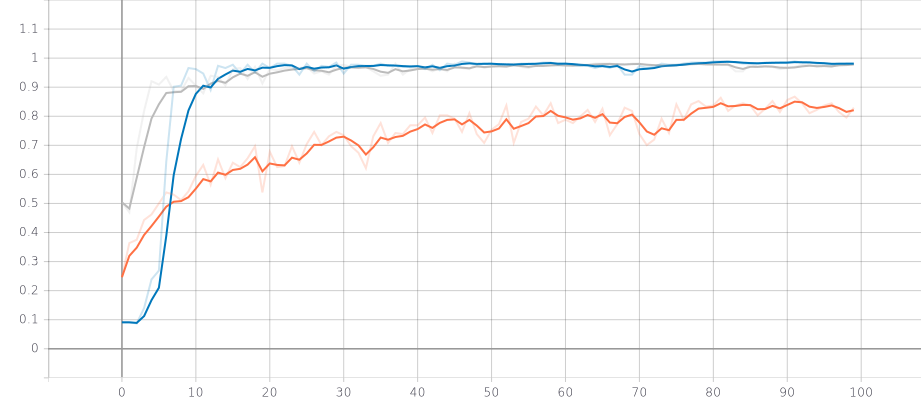
\includegraphics[scale=0.3]{grafiken/rnn-comp.png}
    \caption{Vergleich der Klassifizierungsgenauigkeiten in Abhängigkeit der Epoche. Enthalten sind das gewöhnliche RNN (Orange), LSTM (Grau) und GRU (Blau)}
    \label{gra:rnn-comp}
\end{figure}

Allgemein lässt sich somit sagen, dass nach den in dieser Forschungsarbeit untersuchten Kriterien die GRU Architektur mit einer Klassifikationsgenauigkeit von 89,11\% und einer Trainingsdauer von 18 Minuten und 2 Sekunden die besten Ergebnisse zwischen den RNN-Architekturen liefert.

\section{Vergleich zwischen gewöhnlichen Klassifikatoren und RNN}
\label{subsec:rnn-other-comp}

Betrachtet man nun abschließend alle untersuchten Klassifikatoren, so zeichnet sich sowohl in der Klassifikationsgenauigkeit als auch in der Trainingsdauer ein Unterschied ab. Während selbst der beste gewöhnliche Klassifizierer, die SVM, in etwa zehn Prozentpunkte schlechter in der Klassifikationsgenauigkeit abschneidet als die beste RNN Architektur, das GRU, so braucht dieser für das Ergebnis weniger als die Hälfte der Trainingsdauer. Ebenfalls zu beobachten ist im Vergleich zwischen den gewöhnlichen Klassifizierern und RNN-Architekturen die Tendenz zu besseren Klassifizierungsgenauigkeiten bei größerer Trainingsdauer. Diese allgemeine Tendenz macht sowohl GRU als auch DT besonders interessant, da diese den Trend brechen und trotz geringerer Trainingsdauer bessere Ergebnisse liefern als die mit ihnen direkt verglichenen Architekturen. Sowohl GRU, die als vergleichsweise junge Architektur noch am Anfang ihrer Optimierung stehen, als auch DT, deren Einsatz in Verbindung mit komplexeren Algorithmen auch im Rahmen der Klassifikation von EMG Signalen bereits gute Ergebnisse hervorbrachte (\cite{gokgoz2015comparison}), haben daher großes Potenzial für die Zukunft der Klassifikation von EMG Signalen.

\begin{table}[h]
    \centering
    \bgroup
    \begin{tabular}{| l | c | c |}
        \hline
        \textbf{Klass.} & \textbf{Acc., \%} & \textbf{Dur., Min.} \\
        \hline
        GRU & \textbf{98,11} & \textbf{18:02}\\ \hline
        LSTM & 98,11 & 58:28 \\ \hline
        RNN & 82,95 & 46:14 \\
        \hline
        \hline
        SVM & \textbf{87,94} & 07:10 \\ \hline
        DT & 87,13 & \textbf{00:15 }\\ \hline
        MLP & 86,14 & 03:01 \\ \hline
        kNN & 82,92 & 02:34 \\
        \hline
    \end{tabular}
    \egroup
    \caption{Ergebnisse der Cross Validation in Hinblick auf Klassifizierungsgenauigkeit und Dauer aller untersuchter Klassifikatoren, unterteilt in den verwendeten Klassifikator (Klass.), die Klassifizierungsgenauigkeit (Acc.) und die Trainingsdauer (Dur.)}
    \label{tab:rnn-comp}
\end{table}

\chapter{Fazit und Ausblick}
\label{chap:fazit}

Kern der Forschungsarbeit war der Vergleich zwischen Rekurrenten Neuralen Netzen und state-of-the-art Klassifikatoren, um einen Referenzwert für weitere Forschung in diesem Bereich zu schaffen. Dabei wurden die Besonderheiten und Problemstellungen, die sich durch die Arbeit mit RNN-Architekturen ergeben, aufgezeigt. Rekurrente Neurale Netze wurden dabei erstmals auf den \glqq Forearm 121 EMG\grqq{} Datensatz angewandt. Hierfür wurde eigens für diese Arbeit eine Implementierung der Architekturen vorgenommen und die Netzwerke anhand des Datensatzes trainiert und ausgewertet. Weiterhin wurden state-of-the-art Klassifikatoren implementiert und mit den untersuchten RNN-Architekturen verglichen. Dabei zeigte sich, dass RNN-Architekturen valide Klassifikatoren für EMG-Daten sind und im Vergleich zu gewöhnlichen Klassifikatoren eine signifikant höhere Klassifikationsgenauigkeit aufweisen. Zwar brauchen ältere RNN-Architekturen wie LSTM das achtfache der Zeit, um eine Steigerung der Klassifikationsgenauigkeit um zehn Prozentpunkte zu gegenüber gewöhnlicher Klassifikatoren zu erzielen, allerdings ermöglichen junge Architekturen wie das GRU gleiche Präzision in einem Drittel der Zeit des LSTM. So lässt sich als Fazit ableiten, dass insbesonders moderne RNN-Architekturen wie die GRU mit einiger Optimierung das Potenzial haben könnten, eine präzise Klassifikation von EMG-Signalen in einer ähnlichen Zeit, jedoch mit einer besseren Klassifikationsgenauigkeit, durchzuführen, als selbst präzise gewöhnliche Klassifikatoren wie die SVM.

Das anfängliche Ziel der Forschungsarbeit und die Frage, wie RNN im Vergleich zu gewöhnlichen state-of-the-art Klassifikatoren klassifizieren, lassen sich nun beantworten. Während klassische RNN-Architekturen teilweise signifikant länger für die Klassifikation brauchten als gewöhnliche state-of-the-art Klassifikatoren, schließt sich nun die Lücke in der Trainingsdauer durch moderne Klassifikatoren wie die GRU langsam.

Das macht moderne RNN-Architekturen zu einem vielversprechenden Forschungsansatz, der in Zukunft in Verbindung mit der Klassifikation von EMG-Signalen weiter erforscht werden sollte. Hier sollte der Schwerpunkt auf modernen Architekturen wie dem GRU liegen, da sich im Training von gewöhnlichen RNN auf Grund von Vanishing und Exploding Gradients häufig Probleme offenbaren, die sich durch Verwendung moderner RNN-Architekturen einfach vermeiden lassen. Gleichzeitig dürfen gewöhnliche Klassifikatoren wie die SVM nicht vernachlässigt werden, da diese in vergleichsweise kurzer Zeit und mit wenigen Hyperparametern häufig bereits vergleichbare Ergebnisse erzielen können. Auch einfache Klassifikatoren wie die Entscheidungsbäume könnten aufgrund ihrer leichten Interpretierbarkeit und guter Klassifikationsgenauigkeit ein interessanter Ansatz für weitere Forschung sein. Sie könnten unter anderem zum Verständnis der Klassifikation von EMG-Signalen beitragen.

Für praktische Anwendungsfälle wie die Prothesentechnik zeigt die Klassifikation durch RNN-Architekturen ein großes Potenzial auf. Zwar ist eine kurze Trainingsdauer für eine praktische Anwendung wichtig, eine hohe Klassifikationsgenauigkeit allerdings essenziell. Somit bieten sich hier die untersuchten RNN-Architekturen gut für weitere Forschung in der Zusammenarbeit mit Anwendern an.

Gleichzeitig ist anzumerken, dass in vorgehenden Untersuchungen teilweise bessere Ergebnisse in der Genauigkeit einiger untersuchter Klassifikatoren wie den SVM oder den gewöhnlichen RNN, erzielt wurden. Diese Ergebnisse könnten weitere Potenziale offenbaren und sollten für zukünftige Forschung miteinbezogen werden.

Konkludierend ist aufbauend auf den Ergebnissen dieser Arbeit zu sagen, dass die Präzision und Geschwindigkeit moderner Klassifikatoren durch weitere Forschung vermutlich bald in der Lage sein wird, die alltäglichen Einschränkungen auf Prothesen angewiesener Menschen nachhaltig zu lösen. 

\selectlanguage{ngerman}

\backmatter
\bibliographystyle{literatur/natdin}
\bibliography{literatur/dnn_ba_bib}
\chapter*{Eidesstattliche Erkl\"{a}rung}
\thispagestyle{empty} Ich versichere, dass ich meine Bachelorarbeit
selbstständig und ohne Benutzung anderer als der angegeben
Hilfsmittel angefertigt habe. Alle Stellen, die wörtlich oder
sinngemäß aus Veröffentlichungen oder anderen Quellen entnommen
sind, sind als solche eindeutig kenntlich gemacht. Die Arbeit ist
in gleicher oder ähnlicher Form noch nicht veröffentlicht und noch
keiner Prüfungsbehörde vorgelegt worden.
\bigskip

\raggedright{Mainz, den 27.08.2020} \bigskip \bigskip \bigskip

Alexander Seidmann

\end{document}